\task{Мощения}
\vspace{-0.7cm}
\centerline{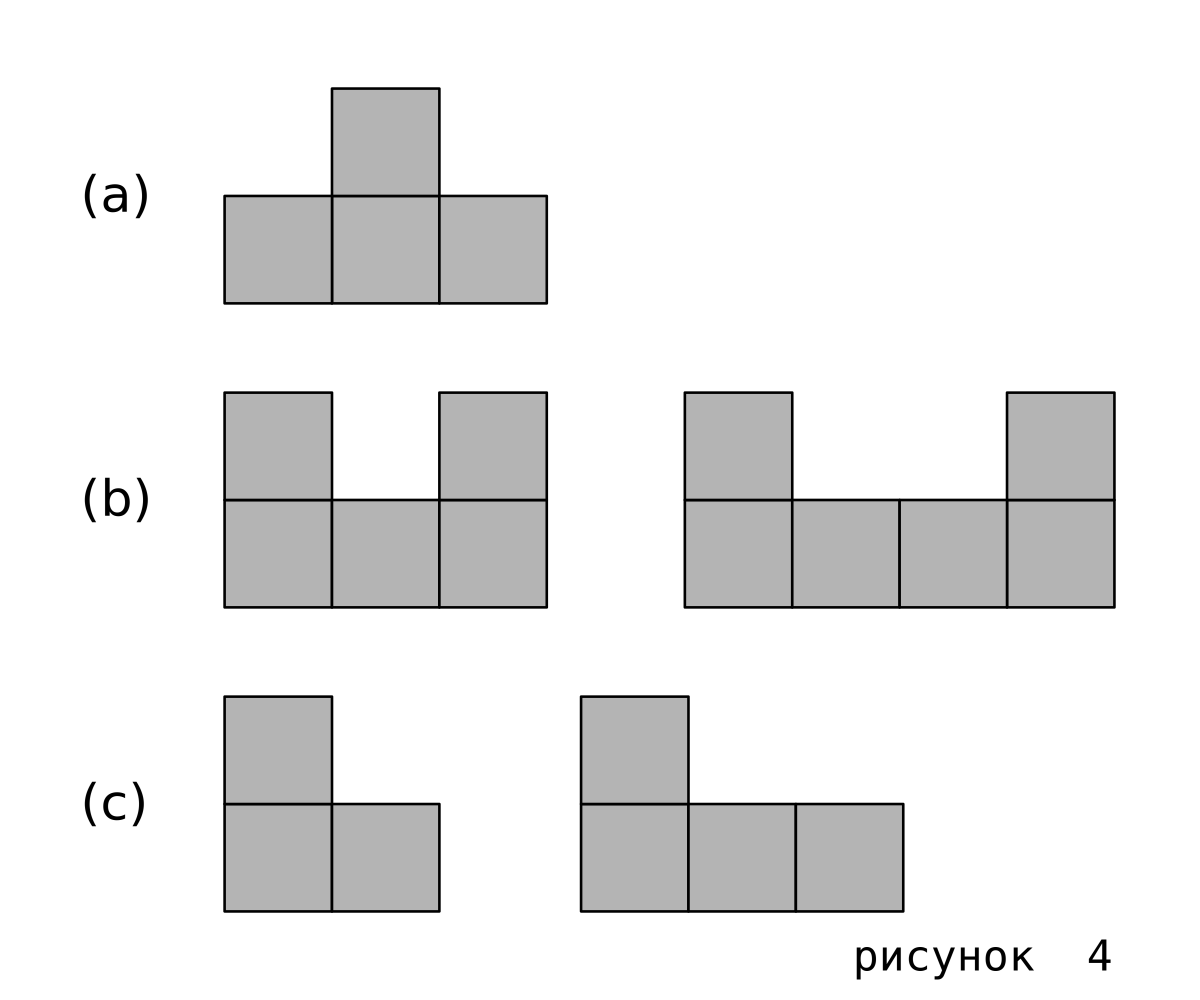
\includegraphics[width=5.5cm]{stats/2018/images/plane-park}}

\begin{enumerate}
\itA Укажите, как замостить плоскость фигурой с рисунка 4{\itshape (a)}.

\itB Укажите способы, которыми можно замостить плоскость каждой из двух фигур на рисунке 4{\itshape (b)}.

\itC Можно ли сложить квадрат какого-либо размера из деревянных\linebreak плиток в форме фигур, изображенных на рисунке 4{\itshape (c)}? При этом необходимо пользоваться плитками обеих форм.
\end{enumerate}